\section{Regularização}
\label{s.regularizacao}

\subsection{\emph{Overfitting}}
\label{ss.overfitting}

Voltemos ao problema de predizer os preços das casas considerando os seguintes exemplos:

  \begin{center}
 	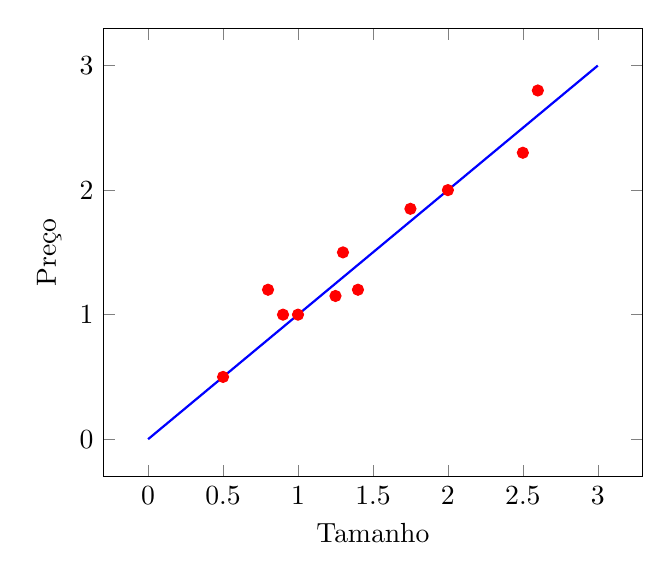
\begin{tikzpicture}[domain=0:3]
  	\begin{axis}[ 
    	xlabel={Tamanho},
    	ylabel={Preço}
  		] 
    	\addplot[blue, thick] {x}; 
    	\addplot[only marks, red] plot coordinates {
        (0.5,0.5)
        (0.9,1)
        (1, 1)
        (0.8,1.2)
        (1.25, 1.15)
        (1.4, 1.2)
        (1.3, 1.5)
        (1.75, 1.85)
        (2, 2)
        (2.5, 2.3)
        (2.6, 2.8)
        
    };
  	\end{axis}
	\end{tikzpicture}
 \end{center}

Podemos perceber que o preço das casas pode não crescer linearmente. Dentro desse espectro de linearidade, nosso modelo pode subtreinar os dados de treinamento.

   \begin{center}
 	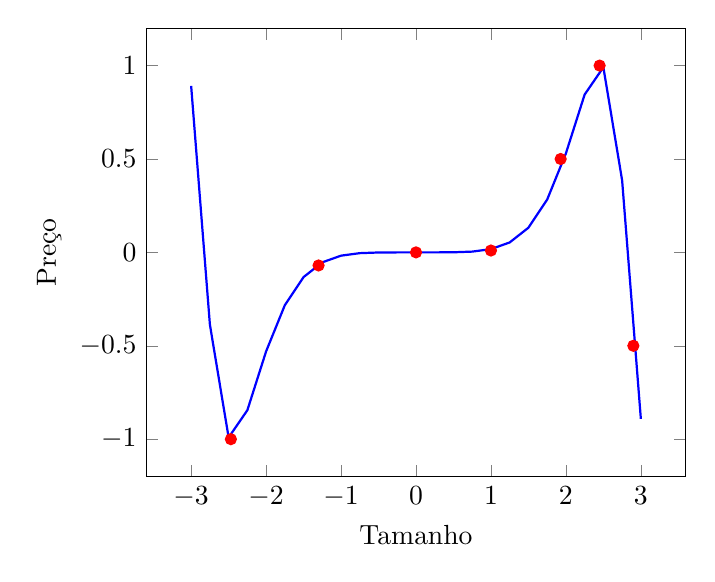
\begin{tikzpicture}[domain=-3:3]
  	\begin{axis}[ 
    	xlabel=Tamanho,
    	ylabel={Preço}
  		] 
    	\addplot[blue, thick] {sin(x^5)};
    	\addplot[only marks, red] plot coordinates {
        (-2.47, -1)
        (-1.3, -0.07)
        (0, 0)
        (1, 0.01)
        (1.93, 0.5)
        (2.45, 1)
        (2.9, -0.5)};
  	\end{axis}
	\end{tikzpicture}
 \end{center}

A função tenta "passar" (adaptar) através de todas as amostras de treinamento, causando o problema de supertreinamento (modelo muito específico).

Portanto, se tivermos muitas características, a hipótese aprendida pode acomodar bem os dados de treinamento ($J(w) \approx 0$), mas também pode falhar em generalizar novos exemplos (predizer os preços de novas casas).

Como podemos checar se tal situação ocorre ou não em nosso modelo? Se tivermos apenas duas características, podemos apenas visualizar o espaço de características. Caso contrário, podemos tentar realizar o seguinte:

\begin{itemize}

\item reduzir a quantidade de características (pode não ser a melhor ideia);
\item regularização: manter todas as características, mas reduzindo os valores dos parâmetros $w_j$ (funciona bem quando possuímos muitas características).
	
\end{itemize}

Suponha que penalizemos e fazemos $w_3$ e $w_4$ muito pequenos:

\begin{equation}
\label{e.small_w}
min_w \frac{1}{2m} \sum\limits_{i=1}^m (h_w(x_i) - y_i)^2 + 1000w_3 + 1000w_4.	
\end{equation}

Com isso, temos que $w_3$ e $w_4 \approx 0$. Na equação acima, se quisermos abrandar a influência de $w_3$ e $w_4$, podemos multiplicá-los por um valor alto (por exemplo $1000$). Basicamente, a ideia é ter valores \textbf{pequenos} para $w = (w_0, w_1, w_2, \dots, w_n)$ para ter uma função de hipótese mais simples (suave).

Basicamente, podemos pegar nossa função de custo (Equação~\ref{eq.mse}) e adicionar um segundo termo à ela, como segue:

\begin{equation}
\label{eq.mse_new}
J(w) = \frac{1}{2m} [\sum\limits_{i=1}^m (h_w(x_i) - y_i)^2 + \lambda\sum\limits_{j=1}^n w_j^2],
\end{equation}

onde $\lambda$ é o parâmetro de regularização que controla a relação entre a não regularização ($\lambda = 0$) e a regularização ($\lambda = \infty$).

\subsection{Regressão Linear Regularizada}
\label{ss.linear_regression_reg}

Nesta seção, iremos discutir sobre a regularização na abordagem de regressão linear. Novamente, nossa ideia é minimizar a Equação~\ref{eq.mse_new}, ou seja, encontrar $w$ o qual minimiza $J(w)$.

Portanto, podemos reescrever o algoritmo do Gradiente Descendente a fim de considerar a Equação~\ref{eq.mse_new} como segue:\\

 repita até convergência \{ \\ \\
 \hspace*{25pt} $w_0 \leftarrow w_0 - \alpha \frac{1}{m} \sum_{i=1}^{m}(h_w(x_i) - y_i) x_i^0$ \\~\\
 \hspace*{25pt} $w_j \leftarrow w_j - \alpha [\frac{1}{m} \sum_{i=1}^{m}(h_w(x_i) - y_i)x_i^j + \frac{\lambda}{m}w_j]$ \\ \\
 \hspace*{15pt} \}\\

Podemos generalizar o problema para uma formulação matricial também:

\[X=
  \begin{bmatrix}
    x_1^0 & x_1^1 & x_1^2 & \dots & x_1^n \\
    x_2^0 & x_2^1 & x_2^2 & \dots & x_2^n \\
    \vdots & \ddots & & & \vdots \\
    x_m^0 & x_m^1 & x_m^2 & \dots & x_m^n \\
  \end{bmatrix}, \in \mathbb{R}^{m\times (n+1)}\] \\
  
\[Y=
  \begin{bmatrix}
    y_1 \\
    y_2 \\
    \vdots \\
    y_m
  \end{bmatrix}, \in \mathbb{R}^{m\times1}\] \\
  
Podemos reescrever a Equação~\ref{e.solution_linear_system} a fim de considerar o termo de regularização:

\begin{equation}
w = (X^TX + \lambda A)^{-1} X^TY
\end{equation}

onde $A$ é uma matriz $(n+1)\times(n+1)$, como segue:

\[A=
  \begin{bmatrix}
    0 & 0 & 0 & \dots & 0 \\
    0 & 1 & 0 & \dots & 0 \\
    0 & 0 & 1 & \dots & 0 \\
    \vdots & & & \ddots & \vdots \\
    0 & 0 & 0 & \dots & 1 \\
  \end{bmatrix}, \in \mathbb{R}^{m\times (n+1)}\] \\
  
\textbf{Exemplo para $n = 2$:}

\[A=
  \begin{bmatrix}
    0 & 0 & 0 \\
    0 & 1 & 0 \\
    0 & 0 & 1 \\
  \end{bmatrix}\] \\
  
A razão para tal situação é garantir que $(X^TX + \lambda A)^{-1}$ seja inversível.

\subsection{Regressão Logística Regularizada}
\label{ss.logistic_regression_reg}

Nesta seção, iremos discutir sobre o classificador de Regressão Logística com o termo de regularização. Podemos reescrever a Equação~\ref{e.general_cost_function} como segue:

\begin{equation}
\label{e.log_regression_new}
-1[\frac{1}{m} [\sum\limits_{i=1}^m y_i log(h_w(x_i)) + (1 - y_1) log(1 - h_w(x_i))]	 + \frac{\lambda}{2m} \sum\limits_{j=1}^n w_j^2.
\end{equation}

Podemos implementar a equação acima considerando o Gradiente Descendente:\\

repita até convergência \{ \\ \\
 \hspace*{25pt} $w_0 \leftarrow w_0 - \alpha(\sum\limits_{i=1}^m(h_w(x_i) - y_i)x_i^0$ \\ \\
 \hspace*{25pt} $w_j \leftarrow w_j - \alpha(\sum\limits_{i=1}^m(h_w(x_i) - y_i)x_i^j + \frac{\lambda}{m}w_j$ \\ \\
 \hspace*{15pt} \}
 
